\documentclass[a4paper,11pt]{article} %%%%%%%%%%%% start of LaTeX file
\usepackage{mathpazo}
\usepackage{tikz}
\usetikzlibrary{shapes}
\oddsidemargin -0.54cm
\textwidth 17.0cm
\textheight 24cm
\topmargin -1.3cm
\parindent 0pt
\parskip 1ex
\pagestyle{empty}
\begin{document} %%%%%%%%%%%% end of LaTeX preamble, start of text
	\medskip\hrule\medskip
	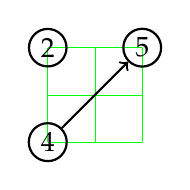
\begin{tikzpicture}[scale=0.6]
	\draw [help lines, color=green] (3,2) grid (5,4) ;
	% coordinate 200 in node (200,1) too large
	\draw [thick] (3,4) node[draw, rounded rectangle] (2) {2};
	% coordinate 200 in node (10,200) too large
	\draw [thick] (3,2) node[draw, rounded rectangle] (4) {4};
	\draw [thick] (5,4) node[draw, rounded rectangle] (5) {5};
	\draw [->, thick] (4) to (5);
	\end{tikzpicture}
	\medskip\hrule\medskip
\end{document}